\documentclass[12pt,a4paper]{article}

\usepackage[english]{babel}
\usepackage[utf8]{inputenc}
\usepackage{amsmath}
\usepackage{amsfonts}
\usepackage{amssymb}
\usepackage{float}
\usepackage{graphicx}
\usepackage{enumitem}
\usepackage[margin=0.8in]{geometry}
\usepackage[justification=centering]{caption}
\usepackage[subnum]{cases}
\setlength{\parindent}{0pt}
\setlength{\parskip}{1em}
\usepackage{empheq}
\usepackage{mlmodern}
\usepackage{amsthm}
\usepackage{listings}
\usepackage{hyperref}
\hypersetup{
    colorlinks=true,
    linkcolor=blue,
    filecolor=magenta,      
    urlcolor=cyan,
}
\usepackage{xcolor} 
\definecolor{codegreen}{rgb}{0,0.6,0}
\definecolor{codegray}{rgb}{0.5,0.5,0.5}
\definecolor{codepurple}{rgb}{0.58,0,0.82}
\definecolor{backcolour}{rgb}{1,1,1}
\lstdefinestyle{mystyle}{
    backgroundcolor=\color{backcolour},   
    commentstyle=\color{codegreen},
    keywordstyle=\color{magenta},
    frame=single,
    numberstyle=\tiny\color{codegray},
    stringstyle=\color{codepurple},
    basicstyle=\ttfamily\footnotesize,
    breakatwhitespace=false,         
    breaklines=true,                 
    captionpos=t,                    
    keepspaces=true,                 
    numbersep=5pt,                  
    showspaces=false,                
    showstringspaces=false,
    showtabs=false,                  
    tabsize=2
}
\lstset{style=mystyle}

\title{\textsc{\large Numerical Assignment\\Condensed Matter Physics (P306)} \\ {\bf\LARGE \vspace{.5em} Wannier Functions\\for a Periodic Potential}}
\author{Gayatri P\\Int. M.Sc. (3rd Year)\\ (2211185)}

\begin{document}
\maketitle
% \tableofcontents

\section{Theory}

Now consider a weak periodic potential perturbation to this Hamiltonian,
\begin{align*}
    H = H_0 + V(x)
\end{align*}
where $V$ is periodic in the lattice space.
\begin{align*}
    V(x+la) = V(x)
\end{align*}
Due to its periodicity, one can also chose to expand $V$ in the Fourier space as
\begin{align*}
    V= \sum_{G} V_G e^{iGx}
\end{align*}
where $G=2\pi x/a$. Now, on solving the Schrodinger's equation, one can obtain the Bloch functions $\psi_q$.
\begin{align*}
    \psi_q(x) = \sum_G C_{q,G} e^{i(q + G)x}
\end{align*}

Once we have the Bloch functions for the lowest energy band, we can construct the Wannier function using,

\begin{align*}
    W(x - R) = \frac{1}{\sqrt{N}} \sum_q \psi_q(x) e^{-ikR}
\end{align*}

where $R$ is a lattice vector ($R = na$, $n \in \mathbb{N}$), $N$ is the number of unit cells in the system
The sum is over all $q$ values in the first Brillouin zone. Let us consider a periodic potential

\begin{align*}
    V(x) = A\cos \left(\frac{2\pi x}{a}\right)
\end{align*}

Similar to the nearly free electron model, the bandgap at the Brillouin zone boundary is $A$, and the Bloch functions near the boundaries can be approximated using

\begin{align*}
    \psi_q(x) \frac{1}{\sqrt{2}} \left(e^{ikx} \pm e^{i\left(k-\frac{2\pi}{a}\right)}x\right) 
\end{align*}

Using these approximate Bloch functions, we can construct the Wannier function. In the following code, for every point $q$, we construct the appropriate Hamiltonian matrix $H_q$ and the calculate the eigenvectors using NumPy. Then, the Wannier function is generated using the above equations and subsequently normalized by dividing it by $\sqrt{N}$. The resulting function is localized around the lattice site $R$, with its shape depending on the strength of the potential $A$. By varying the value of the lattice constant $a$, we can see how the localisation shifts.

% \section{Numerical Modelling of Band Structures}

\section{Implementation}
\subsection{Code}

Below is the Python code used for generating Wannier Functions and plotting them.

\begin{lstlisting}[language=Python, caption=Functions for the construction and generation of WFs]
import numpy as np
import matplotlib.pyplot as plt

def construct_WF(A, a, N=200):
    q_grid = np.linspace(-15* np.pi / a, 15* np.pi / a, N)

    # Construct Hamiltonian matrix for each q
    H_matrices = []
    for q in q_grid:
        H_q = np.zeros((N, N), dtype=complex)
        for i in range(N):
            for j in range(N):
                G_i = 2 * np.pi * i / a
                if i == j:
                    H_q[i, j] = (q + G_i)**2 / 2
                elif abs(i - j) == 1:
                    H_q[i, j] = A / 2
        H_matrices.append(H_q)

    # Calculate eigenvectors for the lowest band
    eigenvectors = []
    for H_q in H_matrices:
        _, eigenvectors_q = np.linalg.eigh(H_q)
        eigenvectors.append(eigenvectors_q[:, 0])  # Lowest energy eigenvector

    # Construct Wannier function
    xs = np.linspace(0, 2, 300)
    wannier_function = np.zeros_like(xs, dtype=complex)
    for i, q in enumerate(q_grid):
        for j, x in enumerate(xs):
            psi_q_x = np.sum(eigenvectors[i] * np.exp(1j * (q + 2 * np.pi * np.arange(N) / a) * x))
            wannier_function[j] += psi_q_x * np.exp(-1j * q * a / 2)

    # Normalization
    wannier_function /= np.sqrt(N)

    return xs, wannier_function
\end{lstlisting}

\begin{lstlisting}[language=Python, caption=Plotting WFs for different values of a]
A = 0.2
a_range = [0.5, 1, 1.5, 2, 2.5, 3]

plt.figure(figsize=(8, 4*len(a_range)))
plt.title(r"Wannier Function for $V(x) = A cos(2\pi x/a)$")

for i in range(len(a_range)):
    plt.subplot(len(a_range)*100 + 10 + i + 1)
    xs, WF = construct_WF(A, a_range[i])
    plt.plot(xs, np.real(WF), '-b', label=f'Re(WF)')
    plt.plot(xs, np.imag(WF), '--r', label=f'Imag(WF)', alpha=0.8)
    plt.ylabel("Re(WF)")
    plt.title(r"a = {0}".format(a_range[i]))
    plt.legend()

plt.xlabel(r"$x$")
plt.show()
\end{lstlisting}

\subsection{Results}

The resultant plots for WF$(x)$ generated are shown below. We are assuming $\hbar = m = 1$ for simplicity.

\begin{figure}[H]
    \centering
    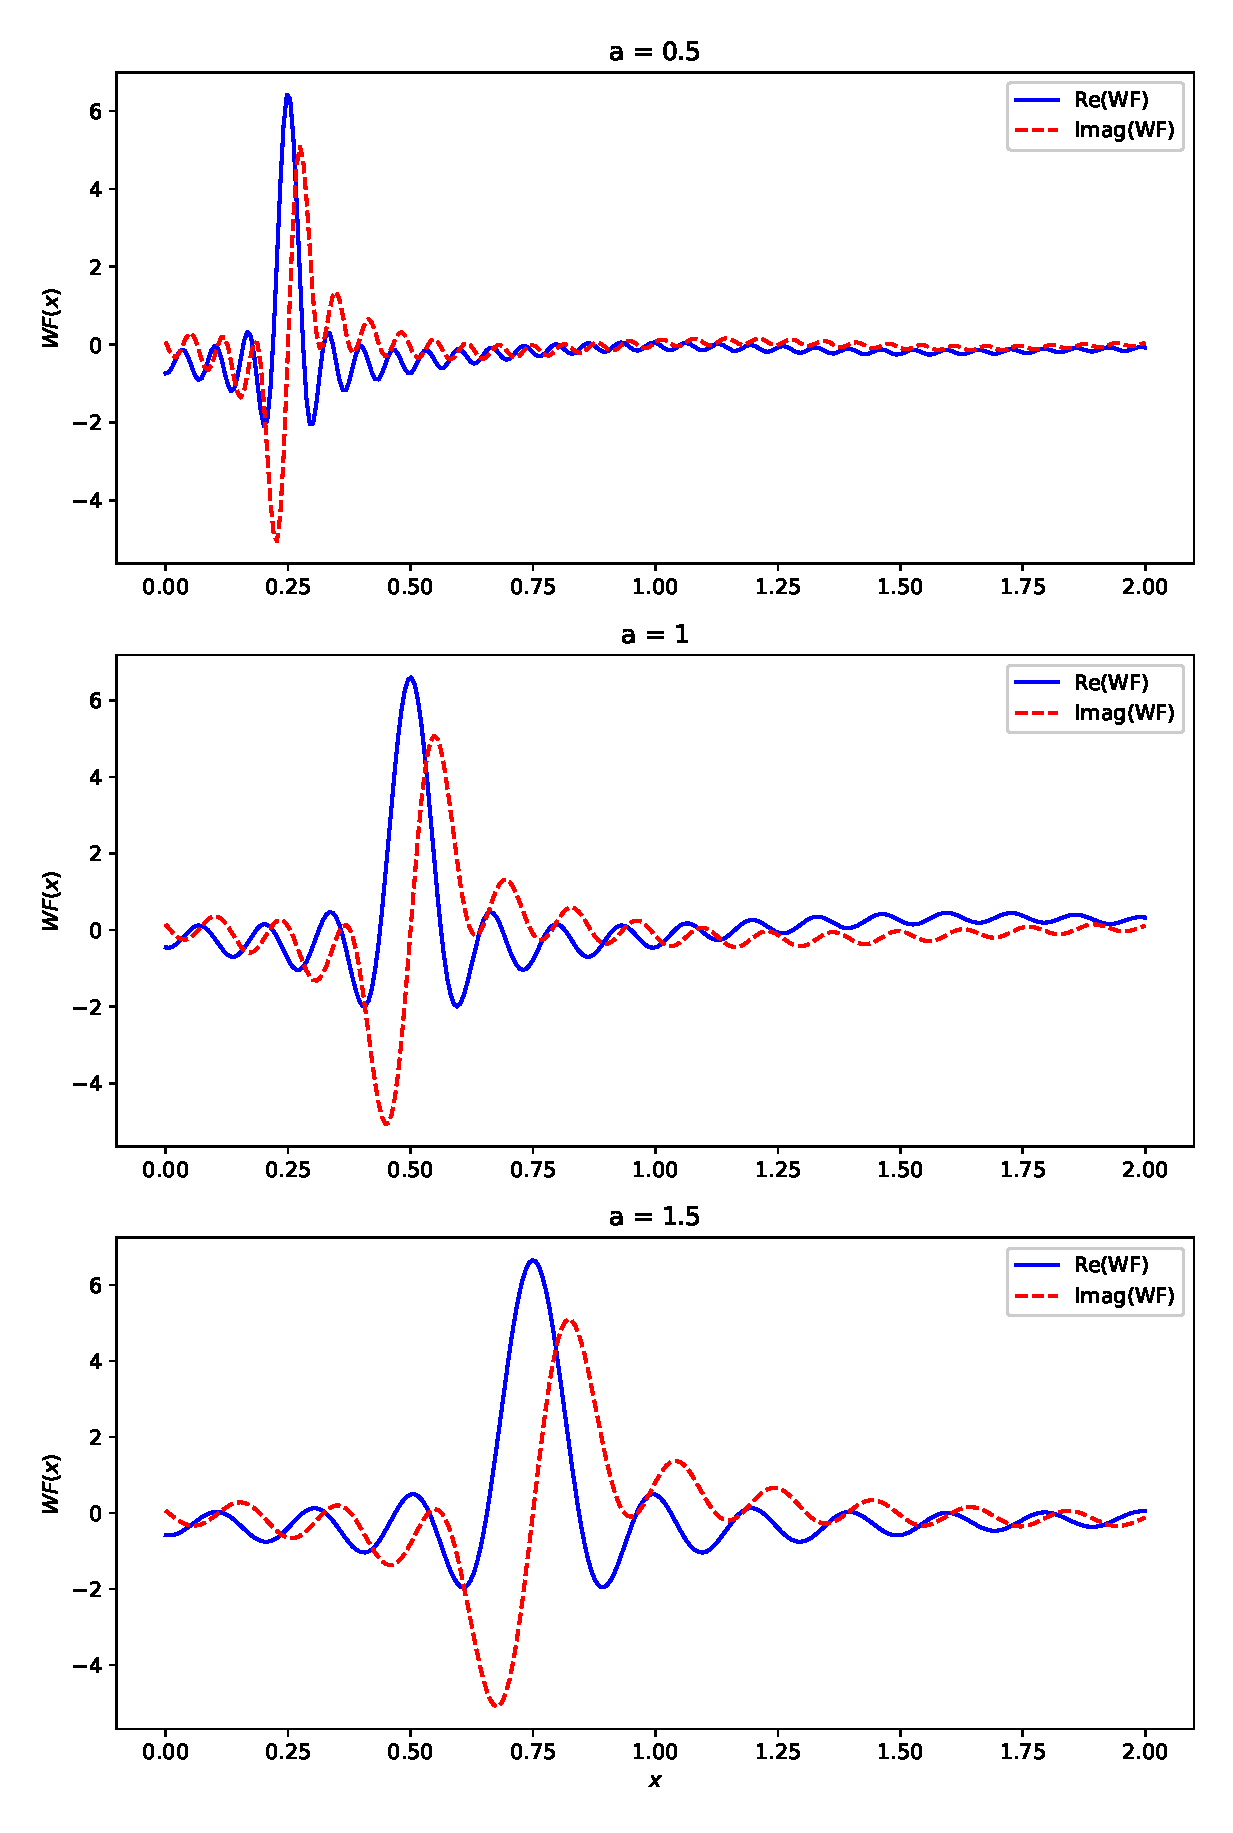
\includegraphics[width=0.9\linewidth]{images/wannier.eps}
    % \caption{Band Structure for when $A=0$ and $B=0$, i.e. a free electron.}
    % \label{1}
\end{figure}

\begin{figure}[H]
    \centering
    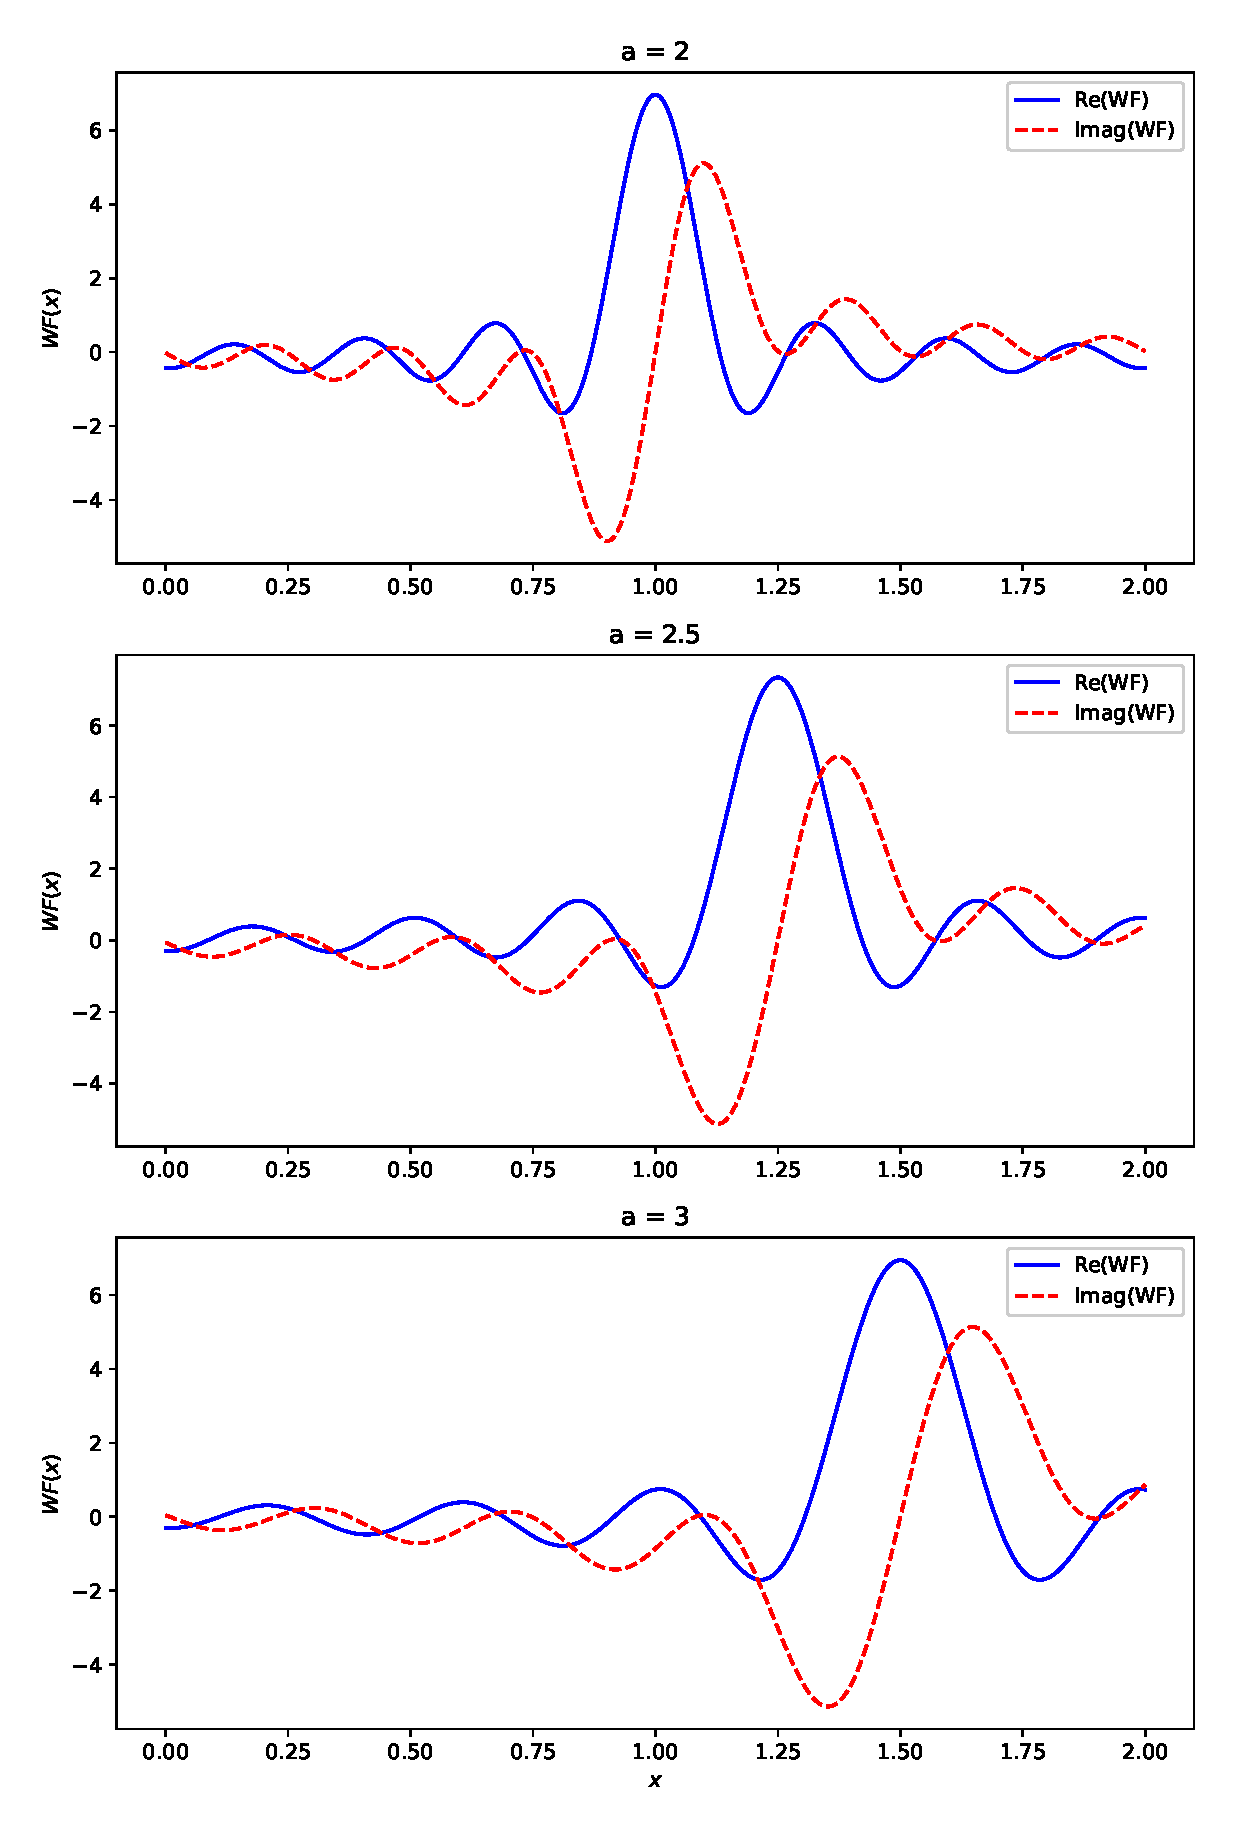
\includegraphics[width=0.9\linewidth]{images/wannier1.eps}
    \caption{The real (and imaginary) parts of the Wannier function plotted against $x$, for different values of the lattice constant $a$.}
    % \label{2}
\end{figure}

\section{Discussion \& Conclusion}
Using Python we were able to numerically generate the localised Wannier functions for a lattice eith periodic potential
\begin{align*}
    V(x) &= A\cos\left(\frac{2\pi x}{a}\right)
\end{align*}
To do this, firstly we generated the Hamiltonian matrix for the potential and solved for its eigenvectors. Using the fourier transform the obtained Bloch functions, we were able to get the required Wannier functions, which were localised at the center of the lattice cell (at $a/2$) as expected.

We see that on increasing the value of $a$, the center of the localisation shifts according to $a/2$. Also, we find that as the lattice constant increases, the resulting spread in the Wannier function also increases. This is expected as now the electron is now less localised due to the increase in the lattice spacing.

We also see that since the wannier function, especially for smaller values of $a$ looks seems to tbe of the form $\frac{\sin x}{x}$. This is because in the limit of small overlap between neighboring orbitals, the orbitals are approximated to be well-localized Gaussian functions. (The Fourier transform of a Gaussian function is also Gaussian). As the corresponding Gaussian functions in q-space becomes very narrow and approaches a delta function, the inverse Fourier transform of that delta function becomes a constant. But since we are considering a periodic system, the inverse Fourier transform becomes a $\frac{\sin x}{x}$ function.
 
\begin{thebibliography}{9}
    \bibitem{a}
    Ashcroft, N. W., \& Mermin, N. D. (1976). \emph{Solid State Physics}. Cengage Learning.
    \bibitem{b}
    Marder, M. P. (2010). \emph{Condensed Matter Physics}. John Wiley \& Sons.
\end{thebibliography}

\end{document}